\documentclass[letterpaper]{article}
\usepackage{typearea}
\typearea{12}
\usepackage{here}
\usepackage{bm}
\usepackage{amsmath, amsfonts}
\usepackage[top=20truemm,bottom=20truemm,left=25truemm,right=25truemm]{geometry}
\usepackage[dvipdfmx]{hyperref,graphicx}
\usepackage{pxjahyper}

% incorporated from Linear Algebra for Everyone 7/18/2022
\newcommand{\bi}[1]{\hbox{\boldmath$#1$}}
\DeclareRobustCommand\transp{^{\mathrm{T}}}
\DeclareMathAlphabet{\cmrv}{OML}{cmm}{b}{it}
\newcommand{\bu}{\hbox{\boldmath$u$}}
\newcommand{\bv}{\hbox{$\cmrv{v}$}}
\newcommand{\bw}{\hbox{\boldmath$w$}}
\newcommand\mat{{\sf MATLAB}}

% prepare to move figures
\graphicspath{ {figs/} }

\begin{document}
\title{The Art of Linear Algebra\\
\vspace{5pt}
\large{
-- Graphic Notes on ``Linear Algebra for Everyone" --
}
}

\author{Kenji Hiranabe
\thanks{twitter: @hiranabe, k-hiranabe@esm.co.jp, \url{https://anagileway.com}} \\
with the kindest help of Gilbert Strang
\thanks{Massachusetts Institute of Technology, \url{http://www-math.mit.edu/\~gs/}}
}

\date{September 1, 2021/updated \today}

\maketitle

\vspace{-5pt}
 
\begin{abstract}
Gilbert Strang 教授の書籍『Linear Algebra for Everyone』
\footnote{``Linear Algebra for Everyone":
\url{http://math.mit.edu/everyone/}日本語は『世界標準MIT教科書 ストラング:教養としての線形代数』(近代科学社)として2023年刊行予定}
の中で紹介されている重要なコンセプトについて,直感的で視覚的な表現を試みた.
ベクトルと行列の計算とアルゴリズムを,行列の積分解の視点から理解する新しい教育教材となることを目的としている.
ここで紹介される行列分解には,行・列分解($\bm{CR}$)ガウスの消去法($\bm{LU}$),
グラム・シュミットの直交化($\bm{QR}$),対称行列の固有値と対角化($\bm{Q \Lambda Q\transp}$),
特異値分解($\bm{U \Sigma V\transp}$)の5分解が含まれる.
\end{abstract}

\section*{Preface}
Kenji Hiranabe による行列操作の図解は,線形代数を理解するのに大変優れた手法である.
初学者は行列の積を「行と列の内積」のように最初理解するが,
見方はそれだけではない.「線形結合」や「ランク1行列」によって線形代数のさらなる理解が深まる.
日本語版にこの図解が掲載されることを嬉しく思う.
\begin{flushright}
-- Gilbert Strang \\ Professor of Mathematics at MIT
\end{flushright}

\tableofcontents

\section{行列の見方 -- 4つ}

まず,行列演算の基礎的な事項から確認して,本記事の視覚的文法に慣れてもらおう.
$m \times n$行列には,「$1$ つの行列」,「$mn$ 個のスカラー」,「$n$ 本の列ベクトル」,「$m$ 本の行ベクトル」
の4つの見方がある.

\begin{figure}[H]
  \centering
  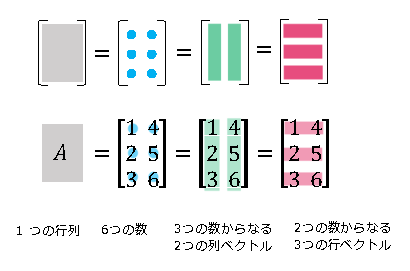
\includegraphics[scale=0.8]{ViewingMatrix-4Ways-j.eps}\\
    \caption{行列の見方 -- 4 つ}
\end{figure}


\begin{equation*}
  A= \begin{bmatrix}
    a_{11} & a_{12}\\
    a_{21} & a_{22}\\
    a_{31} & a_{32}
  \end{bmatrix}
  =
  \begin{bmatrix}
    | & |\\
    \bm{a_1} & \bm{a_2}\\
    | & |
  \end{bmatrix}
  =
  \begin{bmatrix}
    - \bm{a_1^*} -\\
    - \bm{a_2^*} -\\
    - \bm{a_3^*} -
  \end{bmatrix}
\end{equation*} \\

この記事では,列ベクトルはボールドで $\bm{a_1}$ と書く.行ベクトルは,$\bm{*}$ を肩につけて $\bm{a_1^*}$ と書く.
転置されたベクトルと行列は,$\mathrm{T}$ を肩に配置して,それぞれ $\bm{a}\transp, A\transp$ と書く.

\section{2つのベクトルの積}

さて,ここからは書籍『Linear Algebra for Everyone』の当該箇所(以下のように節番号を入れている)を指しながら,
そこで紹介されるコンセプトを紹介していく.詳細は本を見ていただくのがよいが,
できるだけこの記事のみでも理解できるように短い解説を加えた.また,
各図解には,v1(ベクトル同士の積の1番),Mv1(行列とベクトルの積の1番)
のような短い名前が付いており,下の (v1) のように色付き丸で囲って示した.この名前は議論が展開する中で相互参照される.

\begin{itemize}
  \item 1.1 節 ベクトルの線形結合
  \item 1.3 節 行列と列空間 --- ランク1の行列
  \item 1.4 節 行の列積と $A=CR$ \; --- 行方式と列方式
\end{itemize} 


\begin{figure}[H]
  \centering
  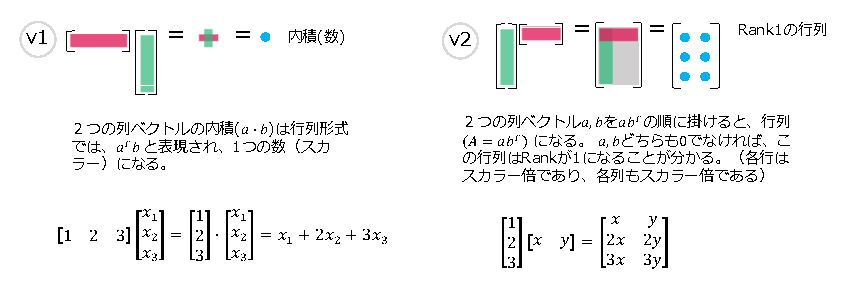
\includegraphics[scale=0.8]{VectorTimesVector-j.eps}
  \caption{2つのベクトルの積 - (v1), (v2)}
\end{figure}

(v1) は基本的な積で,2つのベクトルからスカラーを作る内積と呼ばれる操作だ.
ところが,(v2) のパターンのように行と列を逆順に掛けることもできる(書籍ではこれを外積と呼ぶ).
結果は行列になる.この行列のランクが1であることが分かるだろうか.各行は1行目のスカラー倍になっている(列も同じく).

\section{行列とベクトルの積 -- 2つの見方}

行列とベクトルの積の結果,新しいベクトルが作られる.これを理解するには2通りの見方がある.
1つ1つの成分を,$A$の行ベクトルと列ベクトル$\bm{x}$の内積とする見方(Mv1).
もう1つは,$\bm{x}$を成分ごとにバラして,$A$の列ベクトルの「線形結合」とする見方(Mv2)である.

\begin{itemize}
  \item 1.1節 ベクトルの線形結合
  \item 1.3節 行列と列空間
\end{itemize} 

\begin{figure}[H]
  \centering
  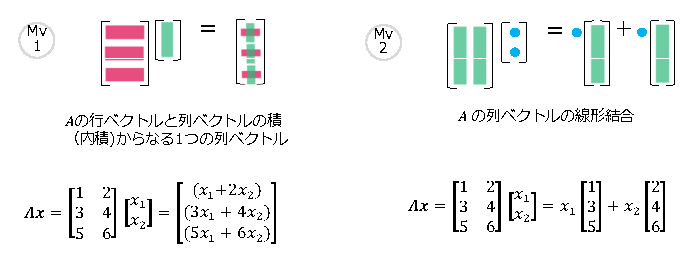
\includegraphics[scale=0.8]{MatrixTimesVector-j.eps}
  \caption{行列とベクトルの積 - (Mv1), (Mv2)}
\end{figure}

初学時は,(Mv1) で積を理解するだろう.しかし,もうひとつの見方 (Mv2) に慣れることで線形代数の理解は
飛躍的に向上する.この見方を使えば,すべての $\bm{x}$ で作られる $A\bm{x}$ によって $A$ の列の線型結合全体が表現されることが分かる.
この積によって生成される部分空間は$A$の列空間と呼ばれ,$\mathbf{C}(A)$ と記述される.
また,$A\bm{x}=\bm{0}$ の解全体となる部分空間は$A$の零空間と呼ばれ,$\mathbf{N}(A)$ と記述される.
零空間を理解するには,(Mv1)の右辺を$\bm{0}$とする.$A$の各行と$\bm{x}$の内積がすべて $0$ すなわち,行空間と直交する空間である.

同様に,(vM1) と (vM2) によって,行ベクトルと行列の積も捉えることができる.

\begin{figure}[H]
  \centering
  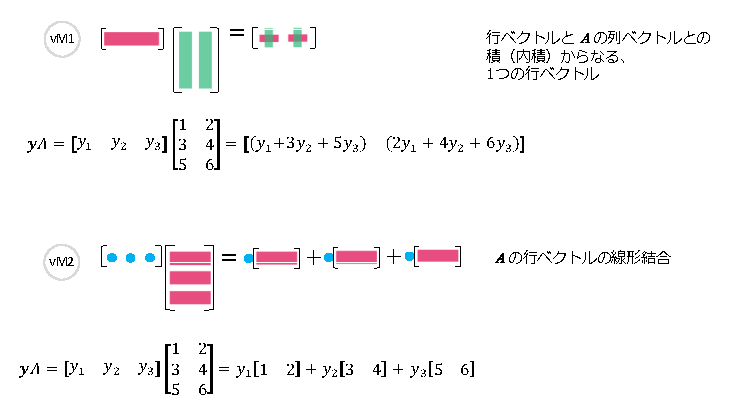
\includegraphics[scale=0.8]{VectorTimesMatrix-j.eps}
  \caption{ベクチョルと行列の積 - (vM1), (vM2)}
\end{figure}

(vM2)の積によって生成される部分空間(を列ベクトルにしたもの)は,$A$の行空間と呼ばれ,$\mathbf{C}(A\transp)$ と記述される.
また,$\bm{y}A=0$ ($A\transp \bm{y}\transp=0$)の解全体となる部分空間(を列ベクトルにしたもの)は
$A$の左零空間と呼ばれ,$\mathbf{N}(A\transp)$ と記述される.(vM1)の右辺を$\bm{0}$とすることによって,
列空間と直交する空間であることが分かる.

本書の最初のハイライトである「4つの基本部分空間」は, $\mathbb{R}^n$ を2つの直交する部分空間で直和分解する
$\mathbf{N}(A)$ + $\mathbf{C}(A\transp)$ と,$\mathbb{R}^m$を2つの直交する部分空間で直和分解する
$\mathbf{N}(A\transp)$ + $\mathbf{C}(A)$ からなる.

\begin{itemize}
  \item 3.5節 4つの基本部分空間の次元
\end{itemize} 

\begin{figure}[H]
  \centering
  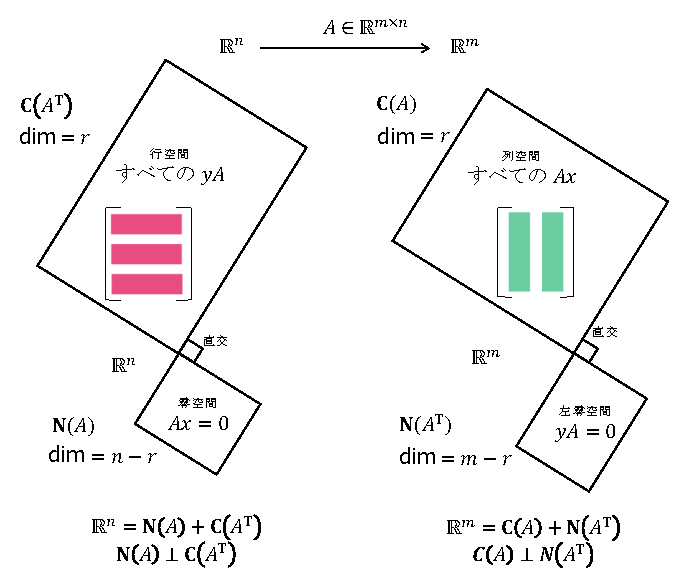
\includegraphics[scale=1.0]{4-Subspaces-j.eps}
  \caption{4つの基本部分空間}
\end{figure}

ランクについては,行ランクと列ランクが等しいことを示す $A=CR$ 分解(6.1)参照.

\section{2つの行列の積 -- 4 つの見方}

前の「行列とベクトルの積」から,自然に「行列と行列の積」が導かれる.

\begin{itemize}
  \item 1.4 節 行列の積と $A=CR$ \; --- 積 $AB=C$ の4つの見方()
  \item 裏表紙の図も参照
\end{itemize} 


\begin{figure}[H]
  \centering
  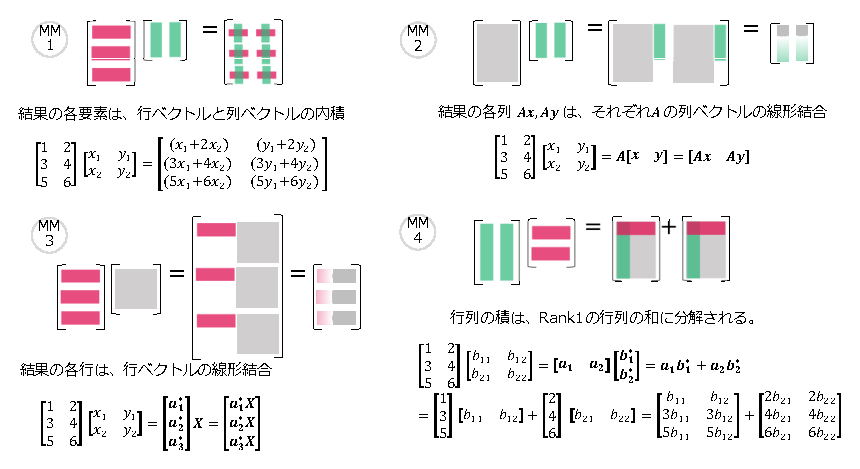
\includegraphics[scale=0.8]{MatrixTimesMatrix-j.eps}
  \caption{2つの行列の積 - (MM1), (MM2), (MM3), (MM4)}
\end{figure}

\section{実用的なパターン}

ここでは,前章の知識を前提として,実用的なパターンを導入する.これによって,
後半の行列の分解をより直感的に理解できるようになる.

\begin{figure}[H]
  \centering
  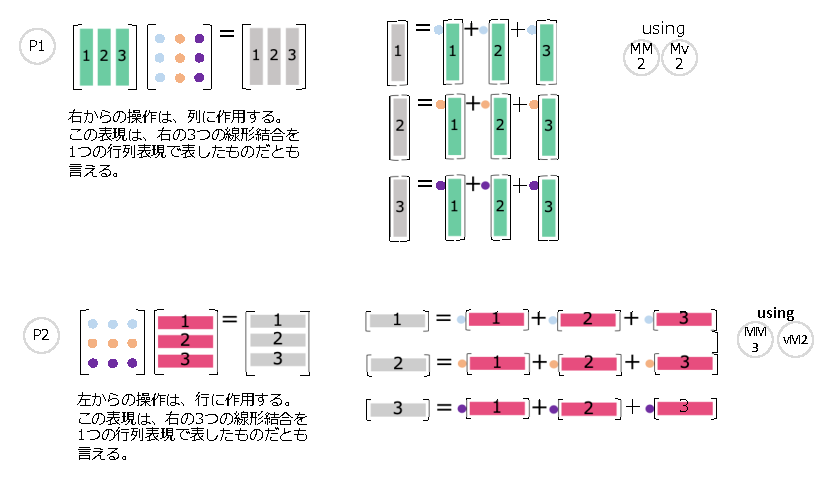
\includegraphics[scale=0.8]{Pattern12-j.eps}
  \caption{パターン 1, 2 - (P1), (P1)}
\end{figure}

(P1)は(MM2)と(Mv2)の組み合わせである.
(P2)は(MM3)と(vM2)の組み合わせである.パターン1が列基本変形(変換行列を右から掛ける),
(P2)が行基本変形(変換行列を左から掛ける)に対応している.
このよく出てくる応用として、次のパターン(P1'), (P2')がある.

\begin{figure}[H]
  \centering
  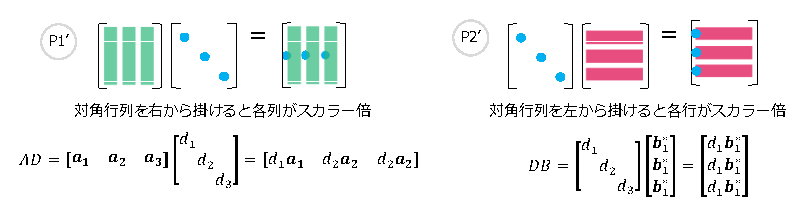
\includegraphics[scale=0.8]{Pattern11-22-j.eps}
  \caption{パターン 1$^\prime$, 2$^\prime$ - (P1$^\prime$), (P2$^\prime$)}
\end{figure}

(P1$^\prime$) では,行列の列に対角のスカラーが掛け算される.一方,
(P2$^\prime$) では,行列の行に対角のスカラーが掛け算される.この2つのパターンは,(P1)と(P2)から派生したものだ.

\begin{figure}[H]
  \centering
  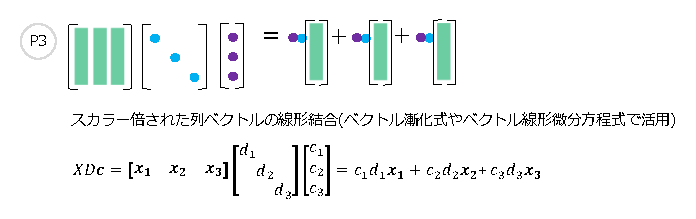
\includegraphics[scale=0.85]{Pattern3-j.eps}
  \caption{パターン 3 - (P3)}
\end{figure}

このパターンは,線形微分方程式や漸化式に対応して頻出する.$XD\bi{c}$ はそれぞれ「解の基底を列ベクトルとする行列」,
「固有値を対角成分に含む対角行列」,「初期値の固有ベクトル方向成分の列ベクトル」である.

\begin{itemize}
  \item 6章 固有値と固有ベクトル
  \item 6.4節 微分方程式への応用
\end{itemize} 

\begin{align*}
  \frac{d \bm{u}(t) }{dt} &= A \bm{u}(t), \quad \bm{u}(0) =\bm{u}_0\\
  \bm{u}_{n+1} &= A \bm{u}_n, \quad \bm{u_0} = \bm{u}_0
\end{align*}

両方の式において,解は $A$ の固有値 ($\lambda_1, \lambda_2, \lambda_3$) と固有ベクトル
$X=\begin{bmatrix} \bm{x}_1 & \bm{x}_2 & \bm{x}_3 \end{bmatrix}$,および,初期値
$\bm{u}(0)=\bm{u}_0$ で決定される係数$\bm{c}=(c_1, c_2, c_3)$ によって表現することができる.
$\bm{c}$は $X$ を基底としたときの初期値 $\bm{u}_0$ の成分(座標)である.

\begin{equation*}
  \bm{u}_0 = c_1 \bm{x}_1 + c_2 \bm{x}_2 + c_3 \bm{x}_3
\end{equation*}
\begin{equation*}
  \bm{c} =
  \begin{bmatrix}
    c_1\\
    c_2\\
    c_3
  \end{bmatrix} = X^{-1} \bm{u}_0
\end{equation*}

微分方程式と漸化式の解は,以下のように簡潔に表現できる.

\begin{align*}
  \bm{u}(t) &= e^{At} \bm{u}_0 = X e^{\Lambda t} X^{-1} \bm{u_0} &= X e^{\Lambda t} \bm{c} &= c_1 e^{\lambda_1 t} \bm{x}_1 + c_2 e^{\lambda_2 t} \bm{x}_2 + c_3 e^{\lambda_3 t} \bm{x}_3\\
  \bm{u}_n &= A^n \bm{u}_0 = X \Lambda^n X^{-1} \bm{u_0} &= X \Lambda^n \bm{c} &= c_1 \lambda_1^n \bm{x}_1 + c_2 \lambda_2^n \bm{x}_2 + c_3 \lambda_3^n \bm{x}_3
\end{align*}

$XDc$ を理解するために,Figure 9 のパターン3(P3) を再度見よ.

\begin{figure}[H]
  \centering
  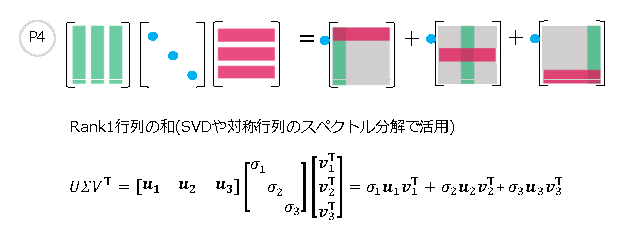
\includegraphics[scale=0.8]{Pattern4-j.eps}
  \caption{パターン 4 - (P4)}
\end{figure}

このパターン(P4) は,固有値分解と特異値分解(SVD)の両方で役に立つ.
これらの行列分解は,「対角行列を中央に挟んだ3つの行列の積」として表現されるとともに,
「固有値や特異値を係数とするランク1行列の和」としても表現できる.

行列の分解については次の節でより詳しく解説する.

\clearpage

\section{5つの行列分解}

\begin{itemize}
  \item 序文  -- 本書のロードマップ
\end{itemize}
$A=CR, A=LU, A=QR, A=Q \Lambda Q\transp, A=U \Sigma V\transp$ の5分解を図解しよう.


\begin{table}[h]
  \begin{tabular}{lll}
    \Large{\boldmath $A=CR$} & 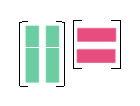
\includegraphics{A_CR.eps} &
    \begin{tabular}{l}
      独立列行列 $C$ と行簡約行列 $R$ の積\\行ランク $=$ 列ランクを示す
    \end{tabular}\\

    \Large{\boldmath $A=LU$} & 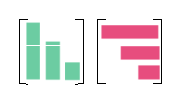
\includegraphics{A_LU.eps} &
    \begin{tabular}{l}
      LU分解 $=$ ガウスの消去法\\下三角行列 $L$ と上三角行列 $U$
    \end{tabular}\\

    \Large{\boldmath $A=QR$} & 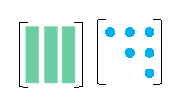
\includegraphics{A_QR.eps} &
    \begin{tabular}{l}
      QR分解 $=$ グラム・シュミットの直交化\\直交行列 $Q$ と三角行列 $R$
    \end{tabular}\\
     
    \Large{\boldmath $S=Q\Lambda Q\transp$} & 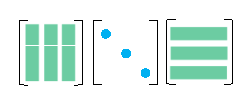
\includegraphics{A_QLQT.eps} &
    \begin{tabular}{l}
      対称行列 $S$ の固有値分解\\固有ベクトル行列 $Q$ と固有値行列 $\Lambda$
    \end{tabular}\\
  
    \Large{\boldmath $A=U\Sigma V\transp$} & 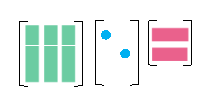
\includegraphics{A_USVT.eps} &
    \begin{tabular}{l}
      どんな長方行列 $A$ にも使える特異値分解\\特異値行列 $\Sigma$
    \end{tabular}
  \end{tabular}
  \caption{5つの行列分解}
\end{table}

% \begin{figure}[H]
%   \centering
%   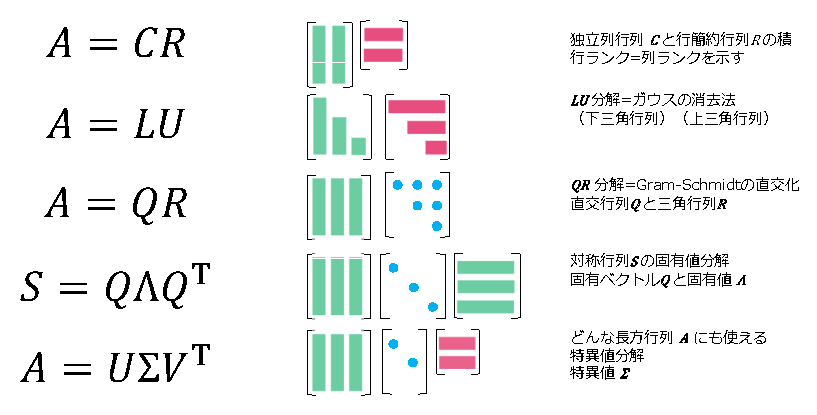
\includegraphics[scale=0.8]{5-Factorizations-j.eps}
%   \caption{5つの行列分解}
% \end{figure}

\subsection{$\boldsymbol{A=CR}$}

\begin{itemize}
  \item 1.4 行列の積と $A=CR$
  \item 付録:$CR$ 分解
\end{itemize}

長方形行列を含む一般の行列 $A$ の行ランクと列ランクは等しい.
$A=CR$ 分解は,この定理をもっとも直感的に示すことができる.
$C$ は$A$の線形独立な列のみからなり,$R$ は $A$の行簡約階段行列(から0のみの行を除いたもの)である.
$A=CR$ によって,$A$ は $r$本の線形独立な列$C$と$r$本の線形独立な行$R$の積に分解される.

\begin{equation*}
  \begin{split}
    A &= CR\\
  \begin{bmatrix}
    1 & 2 & 3 \\
    2 & 3 & 5
  \end{bmatrix}
  & =
  \begin{bmatrix}
    1 & 2 \\
    2 & 3
  \end{bmatrix}
  \begin{bmatrix}
    1 & 0 & 1 \\
    0 & 1 & 1
  \end{bmatrix}
\end{split}
\end{equation*}

左から右へと $A$の列を見ていく.これまでに現れた列と線形独立なものを$C$に入れ,他は捨てる.
第1列と第2列は生き残り,第3列は捨てられる(第1列と第2列の和になっている).
$A$ の各列を再生するには,$C$ の各列を組み合わせる.その組み合わせ係数が $R$ の各列に成分として表記されている.

\begin{figure}[H]
  \centering
  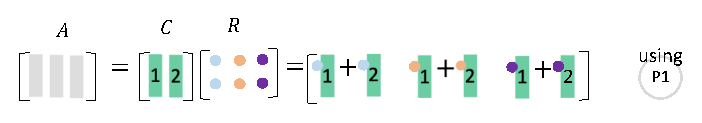
\includegraphics[scale=0.8]{CR1-j.eps}
  \caption{$CR$の列ランク}
\end{figure}

$C$の列数が2であるから,列ランクが2である.すなわち,$A$のすべての列は$C$の列の線型結合である.

\begin{figure}[H]
  \centering
  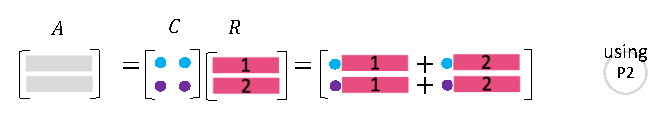
\includegraphics[scale=0.8]{CR2-j.eps}
  \caption{$CR$の行ランク}
\end{figure}

$R$の行数が2であるから,行ランクも2である.すなわち,$A$ のすべての行は$R$の行の線型結合である.

\subsection{$\boldsymbol{A=LU}$}

ガウスの消去法によって $A\bm{x}=\bm{b}$ を解く.この仮定は $LU$ 分解として表現される.
通常,行基本変形行列($E$)を$A$の左から掛けることによって変形し,上三角行列 $U$ を導く.
\begin{align*}
  EA &= U\\
  A &= E^{-1}U\\
L = E^{-1} \text{として} \; , \quad  A &= LU
\end{align*}

すなわち,$A\bm{x}=\bm{b}$ を2ステップで解いている.ステップ1で全身消去 $L\bm{c}=\bm{b}$,ステップ2で後退代入 $U\bm{x}=\bm{c}$ である.

\begin{itemize}
  \item 2.3節 行列計算と $\bm{A=LU}$
\end{itemize}

ここでは,$A$から直接 $L$ と $U$ を計算する.

\begin{equation*}
  A = 
      \begin{bmatrix}
        |\\
        \bm{l}_1\\
        |
      \end{bmatrix}
      \begin{bmatrix}
        -  \bm{u}^*_1  -
      \end{bmatrix}
  +  \begin{bmatrix}
      0 & \begin{matrix} 0 & 0 \end{matrix}\\
      \begin{matrix} 0 \\ 0 \end{matrix} & A_2
    \end{bmatrix}
  = 
  \begin{bmatrix}
    |\\
    \bm{l}_1\\
    |
  \end{bmatrix}
  \begin{bmatrix}
    - \bm{u}^*_1 -
  \end{bmatrix}
  +
  \begin{bmatrix}
    |\\
    \bm{l}_2\\
    |
  \end{bmatrix}
  \begin{bmatrix}
    - \bm{u}^*_2  -
  \end{bmatrix}
  +  \begin{bmatrix}
  0 & 0 & 0\\
  0 & 0 & 0 \\
  0 & 0 & A_3
  \end{bmatrix} = LU
\end{equation*}
 

\begin{figure}[H]
  \centering
  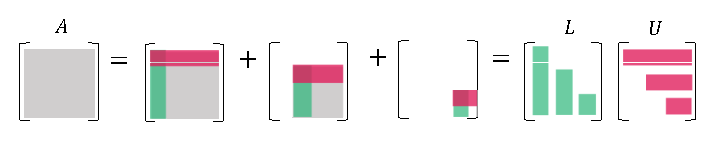
\includegraphics[scale=0.8]{LU1-j.eps}
\caption{再帰的なランク1行列の「皮むき」}
\end{figure}

$L$と$U$を計算するために,まず,$A$の第1行と第1列の外積によって作られるランク1行列の皮をむく.
このランク1行列を $A$ から引き去った残りが $A_2$ である.この過程を$A$に再帰的に適用し,1つずつ
ランク1行列を抜き出していく.

\begin{figure}[H]
  \centering
  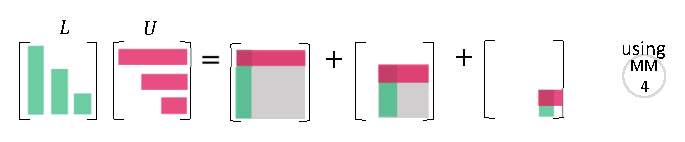
\includegraphics[scale=0.8]{LU2-j.eps}
\caption{$LU$ から $A$ を再生}
\end{figure}

$LU$ から $A$ を再生するプロセスは,より簡単だ.

\subsection{$\boldsymbol{A=QR}$}

$A=QR$ は $A$ の列を直交行列に変換して $Q$ に格納する.
2つの列空間 $\bm{C}(A) = \bm{C}(Q)$ の関係を維持したまま,この変換を行う.

\begin{itemize}
  \item 4.4節 直交行列とグラム・シュミットの直交化
\end{itemize}

グラム・シュミットの直交化では,$\bm{a}_1$ を正規化したベクトル $\bm{q}_1$ がまず選ばれ,
次に,$\bm{a}_2$ を $\bm{q}_1$ との直交成分のみ残して正規化し,それを $\bm{q}_2$ とする.
このプロセスを順に続けていく.

\begin{align*}
  \bm{q}_1 &= \bm{a}_1/||\bm{a}_1|| \\
  \bm{q}_2 &= \bm{a}_2 - (\bm{q}_1\transp \bm{a}_2)\bm{q}_1 , \quad \bm{q}_2 = \bm{q}_2/||\bm{q}_2|| \\
  \bm{q}_3 &= \bm{a}_3 - (\bm{q}_1\transp \bm{a}_3)\bm{q}_1 - (\bm{q}_2\transp \bm{a}_3)\bm{q}_2, \quad \bm{q}_3 = \bm{q}_3/||\bm{q}_3||
\end{align*}

あるいは,$\bm{a}$ を左辺に移動して $r_{ij} = \bm{q}_i\transp \bm{a}_j$ とすると,以下のように記述できる.
\begin{align*}
  \bm{a}_1 &= r_{11}\bm{q}_1\\
  \bm{a}_2 &= r_{12}\bm{q}_1 + r_{22} \bm{q}_2\\
  \bm{a}_3 &= r_{13}\bm{q}_1 + r_{23} \bm{q}_2 + r_{33} \bm{q}_3
\end{align*}

オリジナルの$A$は,直交行列$Q$と上三角行列$R$の積に分解される.

\begin{gather*}
  A = 
  \begin{bmatrix}
    | & | & |\\
    \bm{q}_1 & \bm{q}_2 & \bm{q}_3\\
    | & | & |
  \end{bmatrix}
  \begin{bmatrix}
    r_{11} & r_{12} & r_{13}\\
           & r_{22} & r_{23}\\
           &        & r_{33}
  \end{bmatrix} = QR\\
  \\
  Q Q\transp=Q\transp Q = I
\end{gather*}
\begin{figure}[H]
  \centering
  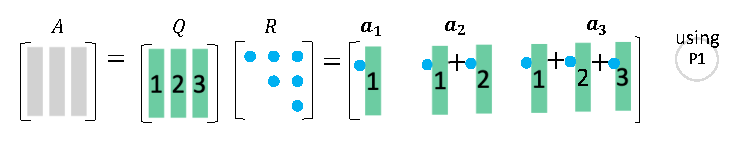
\includegraphics[scale=0.8]{QR-j.eps}
  \caption{$A=QR$}
\end{figure}
$A$ の列ベクトルは,正規直行化された $Q$ の列ベクトルへと変換される.
$A$ の列ベクトルを再生するには,$Q$ と $R$ の掛け算を考えれば簡単である.
ここで,パターン1 (P1) を再度見て視覚的に理解して欲しい.

\subsection{$\boldsymbol{S=Q \Lambda Q\transp}$}

実数成分からなる対称行列 $S$ は,必ず実数固有値と直交する固有ベクトルを持つことが知られている.
この分解で,固有値は$\Lambda$ の対角成分に並び,固有ベクトルは $Q$ の列に配置される.

\begin{itemize}
  \item 6.3節 正定値対称行列
\end{itemize}

\begin{align*}
  S = Q \Lambda Q\transp
&= \begin{bmatrix}
    | & | & |\\
    \bm{q}_1 & \bm{q}_2 & \bm{q}_3\\
    | & | & |
  \end{bmatrix}
  \begin{bmatrix}
    \lambda_1 \\
           & \lambda_2 & \\
           & & \lambda_3
  \end{bmatrix}
  \begin{bmatrix}
  - \bm{q}_1\transp -\\
  - \bm{q}_2\transp -\\
  - \bm{q}_3\transp -
  \end{bmatrix}\\
  \\
  &=
  \lambda_1 \begin{bmatrix}
    |\\
    \bm{q}_1\\
    |
  \end{bmatrix}
  \begin{bmatrix}
    - \bm{q}_1\transp - 
  \end{bmatrix}
  +
  \lambda_2 \begin{bmatrix}
  |\\
  \bm{q}_2\\
  |
  \end{bmatrix}
  \begin{bmatrix}
  - \bm{q}_2\transp -
  \end{bmatrix} 
  +
  \lambda_3 \begin{bmatrix}
    |\\
    \bm{q}_3 \\
    |
  \end{bmatrix}
  \begin{bmatrix}
    - \bm{q}_3\transp -
  \end{bmatrix} \\
&= \lambda_1 P_1 + \lambda_2 P_2 + \lambda_3 P_3
\end{align*}

\begin{equation*}
  P_1=\bm{q}_1 \bm{q}_1\transp, \quad P_2=\bm{q}_2 \bm{q}_2\transp, \quad P_3=\bm{q}_3 \bm{q}_3\transp
\end{equation*}


\begin{figure}[H]
  \centering
  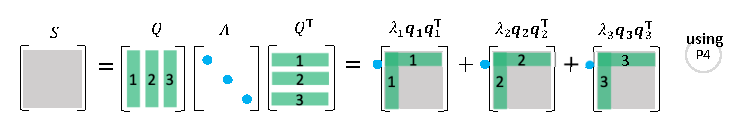
\includegraphics[scale=0.8]{EVD-j.eps}
  \caption{$S=Q \Lambda Q\transp$}
\end{figure}

対称行列 $S$ は,固有値対角行列 $\lambda$ と直交行列 $Q$ の積に分解される.
さらに,ランク1の射影行列 $P=qq\transp$ の線形結合の和としても分解される.
これが「スペクトル定理」である.

\begin{gather*}
  S=S\transp = \lambda_1 P_1 + \lambda_2 P_2 + \lambda_3 P_3\\
  QQ\transp = P_1 + P_2 + P_3 = I \\
  P_1 P_2 = P_2 P_3 = P_3 P_1 = O\\
  P_1^2 =P_1=P_1\transp, \quad P_2^2=P_2=P_2\transp, \quad P_3^2=P_3=P_3\transp
\end{gather*}

\subsection{$\boldsymbol{A=U \Sigma V\transp}$}

\begin{itemize}
  \item 7.1節 特異値分解
\end{itemize}

長方行列を含むすべての行列は,特異値分解(SVD)することができる.
$A=U \Sigma V\transp$ という分解によって,$A$ の左右の特異ベクトルが $U, V$ の列に並び,
対応する特異値は対角行列 $\Sigma$ の対角成分に並ぶ.以下は,簡約形のSVDである.

\begin{figure}[H]
  \centering
  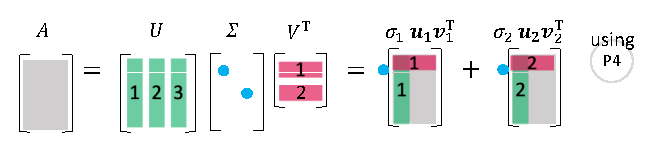
\includegraphics[scale=0.8]{SVD-j.eps}
  \caption{$A=U \Sigma V\transp$}
\end{figure}

$V$ は $\mathbb{R}^n$ の正規直交基底($A\transp A$ の固有ベクトル)であり,
$U$ は $\mathbb{R}^m$ の正規直交基底($AA\transp$ の固有ベクトル)である.
これら2つの基底によって,$A$ は $\Sigma$ へと対角化される.また,
これを展開すると「ランク1行列の線型結合」としても表現できる.

\begin{align*}
  A = U \Sigma V\transp =
  \begin{bmatrix}
    | & | & |\\
    \bm{u}_1 & \bm{u}_2 & \bm{u}_3\\
    | & | & |
  \end{bmatrix}
  \begin{bmatrix}
    \sigma_1 \\
           & \sigma_2 \\
           & &
  \end{bmatrix}
  \begin{bmatrix}
  - \bm{v}_1\transp -\\
  - \bm{v}_2\transp -
  \end{bmatrix}
  & =
  \sigma_1 \begin{bmatrix}
    |\\
    \bm{u}_1\\
    |
  \end{bmatrix}
  \begin{bmatrix}
    - \bm{v}_1\transp - 
  \end{bmatrix}
  +
  \sigma_2 \begin{bmatrix}
  |\\
  \bm{u}_2\\
  |
  \end{bmatrix}
  \begin{bmatrix}
  - \bm{v}_2\transp -
  \end{bmatrix} \\
& = \sigma_1 \bm{u}_1 \bm{v}_1\transp + \sigma_2 \bm{u}_2 \bm{v}_2\transp
\end{align*}

ここで,以下の関係に注意する.

\begin{align*}
  U U\transp &= I_m \\
  V V\transp &= I_n
\end{align*}

この視覚的表現として,パターン4 (P4) を参照して欲しい.

\section*{まとめと謝辞}

この小記事では,初学者が混乱しやすい行列とベクトル演算について,システマティックな視覚表現を試みた.
また,それらを利用して「5つの行列分解」の視覚的理解へ適用した.楽しく読んで頂けたら嬉しいし,
これを自身の線形代数の理解や,教育に利用してもらいたい(大学や教育機関で使ってもらえることを想定している).
グラフィックスは gitHub 上に,Creative Commons Zero v1.0 Universal ライセンスで公開してあり,
.pptx や .eps のフォーマットでも活用できる\footnote{https://github.com/kenjihiranabe/The-Art-of-Linear-Algebra/}. 

Ashley Fernandes から本記事のフォーマットを美しくするプロフェッショナルなアドバイスを頂いた.
また,``Linear Algebra for Everyone" の著者である Gilbert Strang 教授は,
線形代数の新しい教育方法をビデオや本で展開しており,
各コンセプトの直感的な把握によって工学部やデータサイエンスでの実用性を重視したコンテンツを多く手がけている.
記事の細部に渡りアドバイスを頂いた教授に感謝する.

\section*{参考文献と関連記事}
\begin{enumerate}
  \item 
  Gilbert Strang(2020),\emph{Linear Algebra for Everyone}, Wellesley Cambridge Press.,\\
  『世界標準MIT教科書 ストラング:教養としての線形代数』(近代科学社)2023年刊行予定, \\
  \href{http://math.mit.edu/everyone}{http://math.mit.edu/everyone}
  \item
  Gilbert Strang(2016), \emph{Introduction to Linear Algebra},Wellesley Cambridge Press, 5th ed.,\\
  『世界標準MIT教科書 ストラング:線形代数イントロダクション』(近代科学社),\\
  \href{http://math.mit.edu/linearalgebra}{http://math.mit.edu/linearalgebra}
  \item Kenji Hiranabe(2021), \emph{Map of Eigenvalues}, An Agile Way(blog),\\
  \href{https://anagileway.com/2021/10/01/map-of-eigenvalues/}{https://anagileway.com/2021/10/01/map-of-eigenvalues/}\\
  \begin{figure}[H]
    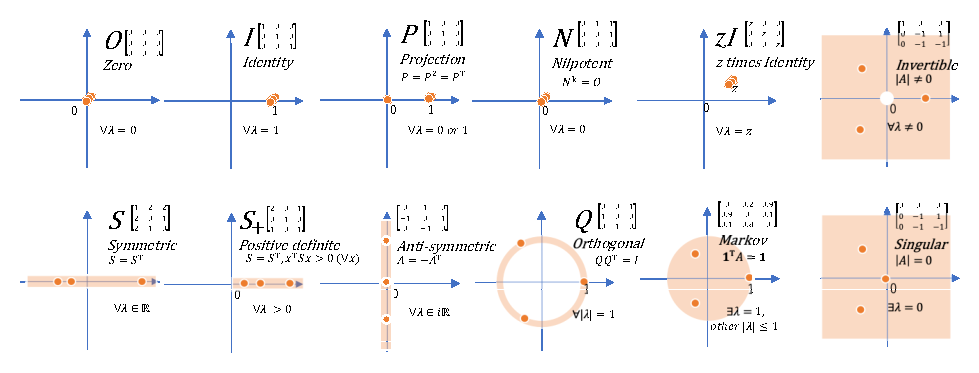
\includegraphics[keepaspectratio, width=\linewidth]{MapofEigenvalues-j.eps}
    \caption{固有値の地図}
  \end{figure}
  \item Kenji Hiranabe(2020), \emph{Matrix World}, An Agile Way(blog),\\
  \href{https://anagileway.com/2020/09/29/matrix-world-in-linear-algebra-for-everyone/}{https://anagileway.com/2020/09/29/matrix-world-in-linear-algebra-for-everyone/}\\
  \begin{figure}[H]
    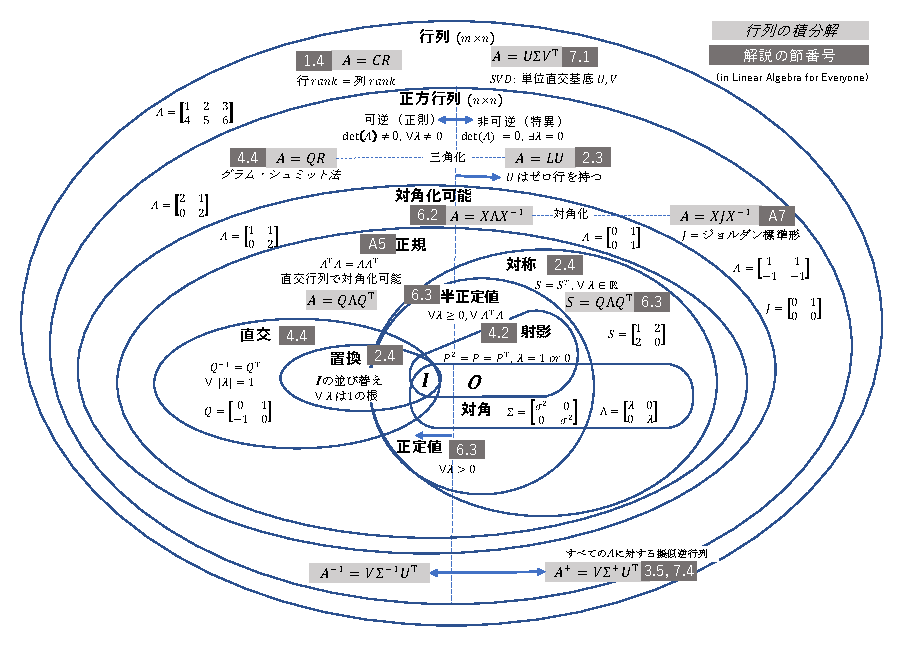
\includegraphics[keepaspectratio, width=\linewidth]{MatrixWorld-j.eps}
    \caption{Matrix World}
  \end{figure}
  \item Kenji Hiranabe, \emph{ストラング先生から学んだ線形代数}, Qiita(blog),\\
  \href{https://qiita.com/kenjihiranabe/items/bfa9cd68bb355afc56b7}{https://qiita.com/kenjihiranabe/items/bfa9cd68bb355afc56b7}\\
 \end{enumerate}
\end{document}
